\documentclass{article}
\usepackage{graphicx}
\usepackage{listings}
\usepackage{amssymb}
\usepackage{amsmath}
\usepackage[utf8x]{inputenc}
\usepackage[english]{babel}
\usepackage{hyperref}
\usepackage{xr}
\usepackage{xcite}
\externalcitedocument{Thesis}

\newtheorem{theorem}{Theorem}[section]
\newtheorem{lemma}[theorem]{Lemma}
\newtheorem{proposition}[theorem]{Proposition}
\newenvironment{proof}[1][Proof]{\begin{trivlist}
\item[\hskip \labelsep {\bfseries #1}]}{\end{trivlist}}
\newcommand{\qed}{$\blacksquare$}

\externaldocument{ch1}
\externaldocument{ch1-5}
\externaldocument{ch2}

\begin{document}

\title{Réponse aux remarques de Jean-Christophe Poudou}
\author{Alexis Bergès}

\maketitle

Les chapitres sont mieux reliés les uns aux autres, avec des résumés plus exhaustifs de leur contribution, des paragraphes de liaison en début et en fin de chaque chapitre, et des références aux terminologies des autres chapitres dans le corps du texte sur les questions d'incertitude notamment.\\

Le code utilisé dans le chapitre 3 est maintenant joint en annexe de la thèse.\\

Conclusion ajoutée, et beaucoup de typos corrigées.\\

\section{Introduction}
\begin{itemize}
\item \textbf{Évoquer la litterature sur le pricing en temps réel de l'électricité.}\\

Ajout dans le dernier paragraphe avant la section ``Contribution'':

\begin{quote}
Some papers have tried to estimate their values empirically, \cite{wolak2007quantifying} and more recently \cite{reguant2011welfare}. There is also a strand of litterature concerned with ramping costs, looking at the optimal price that allows to maximize the overall social welfare \cite{tanaka2006real}, that is, which price schedule allows to maximize the consumer welfare from which the production costs are substracted. This litterature does not use game-theoretical, but concerns itself with the best price signal to use in order to limit the ramping costs incurred due to varying demand, while still considering that the trajectory of demand is known. To our knowledge, there is no game-theoretical framework that has been brought to take ramping costs into account, and describe their effects on optimal strategies for the agents bidding on the market. 
\end{quote}

\end{itemize}

\section{Chapitre 1}
\begin{itemize}
\item \textbf{Modifier la figure \ref{figdyn1} pour la rendre plus claire.}\\

Voici la nouvelle version:

\begin{quote}
\begin{figure}[h] 
\centering
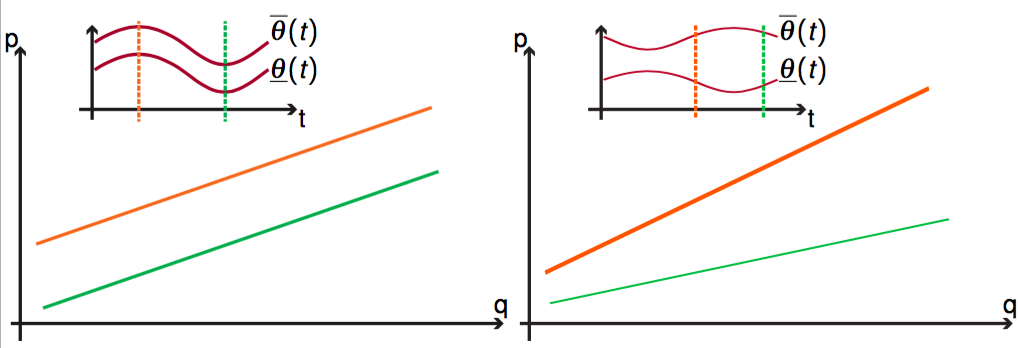
\includegraphics[width=12cm]{figch1/uncertainty.png}
\caption{\small{On the left, this graph plots an envelope of constant width $\omega(t)$ but varying average. The insert represent this envelope, while the graph itself represents the supply curves associated with the points in time represented by the green and orange dotted lines on the insert. On the right, this graph plots an envelope of constant average but varying width $\omega(t)$. }}
\end{figure}
\end{quote}

\item \textbf{Mettre plus en exergue le résultat sur la non ex-post optimalité, détailler la question de la collusion.}\\

La discussion en \ref{discussion_oligo} est maintenant bien plus détaillée. Je n'ai néanmoins pas fait une proposition du résultat sur la collusion, car le résultat ne consiste pas à dire que la collusion est impossible, mais qu'une des caractéristiques des SFE grâce auquel la collusion tacite peut se développer, est l'existence d'un continuum de solutions. Le résultat consiste donc simplement à noter que ce canal n'existe plus avec une solution unique.

\begin{quote}
Most of the tacit collusion concern that is present in the literature is based on the existence of a continuum of solutions \cite{bolle1992supply}. This continuum is thought as being conducive of tacit collusion because the electricity market entails repeated interactions between producers. In this case, producers can be feared to be able to learn to pick the most profitable Nash equilibria. Although a Nash equilibrium is not usually considered conducive to collusion, as each player's strategy is the best response to the other's and there is no profitable deviation, a multiplicity of Nash equilibrium lets open the possibility to pick and choose the most profitable one out of the available options, as compared to the one leading to the strongest competition.\\

Our result implies this pathway for tacit collusion is not available anymore. With only one Nash equilibria at any given time no learning can bring about tacit collusion. This is a strong result about the structure of competition in our framework. The existence of ramping costs leads to a model in which no tacit collusion can exist, suggesting that the policy recommendations about such collusion stemming from the supply function equilibria litterature might be strongly dependent on not taking into account ramping costs.\\

Our solutions are also not ex-post optimal contrary to the traditional results. As our solutions depend explicitly on the structure of the uncertainty around demand shocks, any additional information shifting the expected distribution of shocks would imply a different bid. Ex-post optimality is a very strong result, and, one could argue, more of a quirck from the usual models than its abscence in ours.
\end{quote}

\item \textbf{Mettre en exergue le résultat sur les prix négatifs.}\\

Nouvelle proposition:

\begin{quote}
\begin{proposition}
With $\gamma > 0 $, their exists values of shocks for which the prices are negative. More precisely, their exists negative prices if the following condition on the parameters of the shocks holds:
$$\frac{4\gamma+2+\lambda}{2+\lambda}\frac{1+\lambda}{4\gamma+1+\lambda}b<a<\frac{4\gamma+2+\lambda}{2+\lambda}b$$
\end{proposition}

\begin{proof}
We want the condition under which our solutions exhibit negative prices. First, our supply schedule needs to be positive. Second, for there to exist possible negative prices, one needs the smaller possible price, the one obtained for $\theta=-1$, to be negative.

This can be rewritten as conditions on the shocks, using the expressions from eq. \ref{monopsol} and eq. \ref{monopS}:
\begin{align*}
S*(p(-1))&>0\\
p(-1)+\frac{4\gamma}{2+\lambda}b&>0\\
-a\frac{4\gamma+1+\lambda}{4\gamma+2+\lambda}+ b\frac{1+\lambda}{2+\lambda}&>\frac{4\gamma}{2+\lambda}b\\
a&<\frac{4\gamma+2+\lambda}{2+\lambda}b
\end{align*}
and:
\begin{align*}
p(-1)&<0\\
-a\frac{4\gamma+1+\lambda}{4\gamma+2+\lambda}+ b\frac{1+\lambda}{2+\lambda}&<0\\
a&>\frac{4\gamma+2+\lambda}{2+\lambda}\frac{1+\lambda}{4\gamma+1+\lambda}b
\end{align*} \qed
\end{proof} 
\end{quote}

\item \textbf{Précisions sur le choix du processus stochastique et sur l'équation de Fokker-Planck.}\\

Ajouts suivants dans la section \ref{stoprocess}:

\begin{quote}
A regular candidate for richer stochastic dynamics than a simple brownian process is an Ornstein–Uhlenbeck process. Unfortunately for us, such a process has unbounded support. We are going to use a richer set of stochastic processes: It\={o} processes. 
\end{quote}
et
\begin{quote}
Such a stochastic process has a distribution of probability $f(\theta)$ given by Fokker-Planck's equation, easily solved here. In the general case of an It\={o} process given by SDE \ref{sdegen}, one obtains in \ref{FokP} the generic Fokker-Planck equation for its distribution of probability $f(\theta,t)$. This equation allows, given an initial condition on the distribution of probability of the variable, to observe how this distribution evolves to reach the steady state distribution, that is the limit distribution that any initial condition yields. If one knows the value of the stochastic variable at one point in time, one can use this equation to obtain the spread in its distribution over time. 
\end{quote}

\item \textbf{Clarifier la convergence du modele lorsque les couts dynamiques tendent vers 0 vers la solution obtenue pour un monopole dans le cadre de Klemperer et Meyer.}\\

Ajout de la proposition \ref{monopequilibriaKM}:
\begin{quote}
\begin{proposition}
When taking $\gamma\to 0$, the above solution converges towards the solution obtained in the Klemperer and Meyer framework, which for a monopoly is also unique.
\end{proposition}

\begin{proof}
Consider the following profit:
$$p\cdot D(\theta,p) - C(D(\theta,p))$$
Now take a linear demand schedule $D(\theta,p) = a\cdot \theta + b - p$ and a quadratic cost function $C(D(\theta,p)) = \frac{\lambda}{2} D(\theta,p)^2 = \frac{\lambda}{2}(a\cdot \theta + b - p)^2$.
The F.O.C. with respect to $p(\theta)$ writes:
\begin{eqnarray}
D(\theta,p)  + p\cdot \partial_p D(\theta,p) - C'(D(\theta,p))\partial_p D(\theta,p)  &=&0\\
C'(D(\theta,p)) - \frac{D(\theta,p)}{\partial_p D(\theta,p)} & =&p\\
(1+\lambda)(a\cdot\theta+b-p)&=&p\\
p&=&\frac{1+\lambda}{2+\lambda}(a\cdot\theta+b)\\
\end{eqnarray}
This result is the same as that of proposition  \ref{monopequilibria} with $\gamma \to 0$. \qed
\end{proof} 
\end{quote}

\item \textbf{Clarifier l'hypothèse ``price has to weakly increase with the shocks'' dans la partie \ref{maxprogram}.}\\

Il s'agit de prendre la contrainte sur la courbe d'offre, qui doit croître avec le prix, et d'en déduire un contrainte sur la dépendance du prix avec les chocs. Ajout d'une phrase pour clarifier: 

\begin{quote}
Last, we consider that the shocks $\theta$ are ordered so that the demand is increasing in $\theta$, i.e. $\frac{\partial D}{\partial\theta}\geq0$, and that the price has to weakly increase with the shocks, i.e. $\dot{p}\geq0$, which garanties that the supply function increases with shocks.
\end{quote}

\item \textbf{Clarifier la proposition \ref{gammato0}, pourquoi reste-t-on unique ? }\\

J'ai clarifié en indiquant que cette proposition concerne le cas $\gamma\to0$, avec $\gamma>0$. Il est possible de s'approcher aussi proche que l'on veut de la spécification du modèle de KM, tant que les coûts dynamiques sont non nuls nous conservons le résultat d'unicité. Lorsque les coûts dynamiques sont rigoureusement égaux à 0, nous sommes bien de retour dans le cas de KM. Il ne s'agit pas d'une transition continue entre ces deux comportements.

\begin{quote}
\begin{proposition}
When $\gamma\to0$, with $\gamma>0$, the solution remains unique and converges towards the linear schedule available in KM's set of solutions, that is the same schedule selected with KM's selection rule obtained when considering an infinite support for the shocks.
\end{proposition}
\end{quote}

\item \textbf{Expliquer pourquoi il est désirable que la distribution de probabilité des chocs tende vers 0 aux bornes dans la partie \ref{setupdyn}.}\\

Ajout d'une justification:

\begin{quote}
We also consider that a desirable property is that the distribution reaches 0 continuously at the bounds of its support, because there is no boundary condition on the demand for electricity that would justify that one has a positive probability of reaching a given bound, but a zero probability of reaching an infinitesimally close value to this bound. 
\end{quote}

\end{itemize}

\section{Chapitre 2}
\begin{itemize}
\item \textbf{Détailler l'argument justifiant de l'emploi d'une méthodologie non paramétrique vs une approche cherchant a fitter des fonctions logistiques sur les données.}\\

Plus de détail apporté, notamment en évoquant la métrique que nous avons en tête lorsque nous évoquons que les données ne sont pas bien fittées par une fonction logistique, illustré en fig. \ref{assymetry}, mais aussi en détaillant ce que nous entendons par le fait qu'un fit paramétrique ``mélange'' de l'information de plusieurs parties de la courbe sur un paramètre.

\begin{quote}
Instead, we develop a non-parametric, functional data analysis approach to select comparable data points from the original bid functions. In our case, this selection of points will yield 4 regions for every curves, each region can be thought of as linear. These selected points are comparable across repetitions of the market (i.e. auctions for different hourly contracts) and can then be used to run a cross-sectional reduced form model. The interest of this approach is threefold. First, it aims to use as much of the original information as possible without distorting it into parameters of a logistic function. What we mean by distortion is the example displayed in Fig. \ref{assymetry}, where one can see that the fitted logistic function in green is very far from the data (in the sense that the integral of the absolute value of the difference of the two curves is very large) because the underlying data simply does not have the proper shape. Also, information about different parts of the bid function does not influence one another, contrary to a parametrized form in which one tries to fit a specified function to data. This implies that the error between the functional form and the data at any point of the curve influences the fitted parameters, therefore ``mixing'' information from the whole curve into the choice of a given value for the parameter. Second, our approach is “scalable” because as many points as necessary can be extracted. The cross-sectional analyses are then conditioned on the type of comparable points selected. Third, while our analysis provides support for an underlying tri-linear or S-shaped functional form, we do not need to assume a specific functional form nor impose overly simplistic assumptions, such as symmetry of the functional forms, to ensure convergence of the estimator.\\
\end{quote}

\item \textbf{Comment la production EnR intervient-elle dans le marché ? }\\

Elle est injectée directement dans le réseau sans être pilotable et est donc une production minimale non flexible, elle vient imputer la demande nette adressée aux moyens de production flexibles.

\item \textbf{RTEBlackbox, n'est-ce pas sûrement déjà une estimation basée sur les variables précitées ?}\\

Si, tout à fait, c'est pour cela que nous faisons une regression et que nous ne conservons que les résidus afin d'éviter la collinéarité avec nos variables tout en conservant une potentielle information disponible dans la prévision RTE que nos variables ne capturent pas. Pour clarifier ce point, l'explication est développée p. \pageref{RteBlackBox}. 

\begin{quote}
At the same time, it is evident that this variable uses much of the information that we explicitly control for in the regressions, the variables defined above, therefore in addition to the possibility that we might not have all the variables that go into building this prediction for the hourly consumption, collinearity is an issue. In order to have correct coefficient estimates, we adopt an instrumental variable approach by regressing the RTE prediction on our exogenous factors, extracting the residuals and only including the unexplainable component of the RTE prediction in the demand estimation in the form of a separate variable called RteBlackBox.
\end{quote}
\end{itemize}

\section{Chapitre 3}
\begin{itemize}
\item \textbf{Détailler les autres sources d'incertitude non étudiées.}\\

Ajout de plus de détail dans le deuxième paragraphe du chapitre.

\begin{quote}
We focus on two sources of uncertainty for traditional electricity suppliers, namely uncertainty about the realization of the market demand and uncertainty from the inherently unpredictable meteorological situation
(which affects renewables generation), mainly because those are the two main sources of uncertainty in the span of time covered by our data (2011-2013). There is one blind spot in our analysis: we do not have data about the interconnected countries, which themselves affect the French market, and therefore introduce another important of uncertainty. Not taking this effect into account essentially introduces noise in our data and means that we need more data to infer the significance of an effect compared to a case where we would be able to control for it. We propose a methodology to measure this uncertainty and its impact on firm strategies on the electricity market. 
\end{quote}

\item \textbf{``Given that renewable generation is an exogenous source of supply'' :
Pourtant les suppliers peuvent détenir ces technologies ?}\\

Oui tout à fait, mais ils n'en contrôlent pas le niveau de production, toute production renouvelable est injectée sur le réseau, et en cela cette production est exogène. 
\end{itemize}



\end{document}
